% ==========================================
% BAB II STUDI LITERATUR
% ==========================================
\chapter{STUDI LITERATUR}
\label{chap:studi-literatur}

Bab ini menyajikan tinjauan komprehensif terhadap literatur yang relevan dengan pengembangan sistem rangkuman otomatis berbasis \textit{AI} untuk mereduksi \textit{information overload} dalam komunitas finansial Telegram. Studi literatur ini mencakup tujuh domain utama: (1) \textit{Information Overload} dan \textit{Cognitive Load Theory}, (2) \textit{Text Summarization} dengan \textit{Large Language Models}, (3) Analisis Sentimen untuk Media Sosial Finansial, (4) \textit{Named Entity Recognition} untuk Teks Finansial Indonesia, (5) \textit{Topic Modeling} dengan BERTopic, (6) Telegram sebagai Platform Komunitas, dan (7) Arsitektur Pemrosesan Data \textit{Real-Time}. Setiap domain memberikan landasan teoretis dan metodologis yang mendukung desain, implementasi, dan evaluasi sistem yang dikembangkan dalam penelitian ini.

% ==========================================
\section{\textit{Information Overload} dan \textit{Cognitive Load Theory}}
\label{sec:information-overload}

\textit{Information overload} merupakan fenomena di mana individu dihadapkan pada volume informasi yang melampaui kapasitas kognitif mereka untuk memproses secara efektif \autocite{eppler2004}. Dalam konteks komunitas online, khususnya platform media sosial seperti Telegram, masalah ini menjadi semakin akut karena tingginya laju produksi dan distribusi informasi. Bagian ini mengulas teori-teori fundamental yang menjelaskan bagaimana \textit{information overload} memengaruhi pengambilan keputusan, serta mengidentifikasi strategi mitigasi yang dapat diterapkan melalui sistem otomatis berbasis \textit{AI}.

\subsection{Konsep dan Dampak \textit{Information Overload}}

Penelitian seminal oleh \textcite{eppler2004} menyediakan landasan teoretis yang komprehensif tentang konsep \textit{information overload}. Berdasarkan tinjauan literatur dari berbagai disiplin ilmu termasuk \textit{Organization Science}, Akuntansi, Pemasaran, dan Sistem Informasi Manajemen, mereka mendefinisikan \textit{information overload} sebagai kondisi di mana kualitas pengambilan keputusan menurun ketika kuantitas informasi yang tersedia melampaui kapasitas pemrosesan individu. Studi tersebut mengidentifikasi hubungan inverted U-curve antara kuantitas informasi dan kualitas keputusan, yang menunjukkan bahwa setelah mencapai titik optimal, penambahan informasi justru menurunkan performa kognitif. Temuan ini sangat relevan dengan konteks komunitas Telegram finansial yang menghasilkan ratusan hingga ribuan pesan per hari, yang berpotensi menempatkan anggota komunitas pada sisi kanan kurva tersebut di mana \textit{overload} terjadi.

\begin{figure}[H]
  \centering
  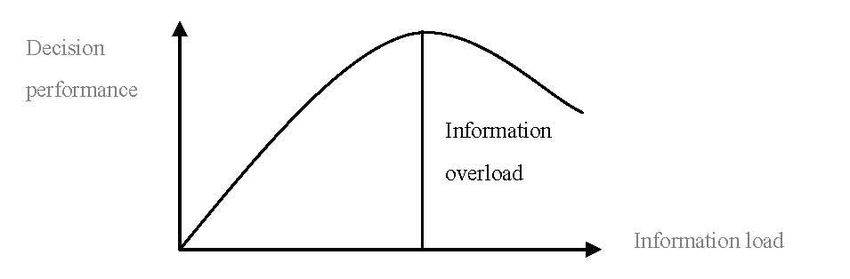
\includegraphics[width=0.7\textwidth]{image/information-overload-curve.png}
  \caption{Hubungan \textit{inverted U-curve} antara kuantitas informasi dan kualitas pengambilan keputusan, menunjukkan titik optimal dan zona \textit{overload} (diadaptasi dari \textcite{eppler2004})}
  \label{fig:info-overload}
\end{figure}

\textcite{shahrzadi2024} memperkuat pemahaman ini melalui \textit{scoping review} terbaru yang menganalisis penyebab, konsekuensi, dan strategi penanganan \textit{information overload}. Penelitian mereka mengidentifikasi tiga kategori penyebab utama: (1) faktor personal seperti keterbatasan kapasitas kognitif dan kurangnya keterampilan manajemen informasi, (2) karakteristik informasi seperti ambiguitas, kompleksitas, dan ketidakpastian, dan (3) parameter teknologi informasi termasuk intensitas notifikasi dan desain antarmuka. Dampak yang diidentifikasi mencakup penurunan produktivitas, kualitas keputusan yang buruk, stres, dan kelelahan kognitif. Yang paling signifikan bagi penelitian ini adalah identifikasi mereka terhadap strategi mitigasi berbasis teknologi, khususnya penggunaan \textit{filtering tools} dan sistem otomatis untuk mereduksi volume informasi, yang memberikan justifikasi langsung untuk pengembangan bot rangkuman otomatis.

\subsection{Landasan Teori: \textit{Cognitive Load Theory}}

\textit{Cognitive Load Theory} (CLT), yang dikembangkan oleh \textcite{sweller1988}, memberikan kerangka teoretis untuk memahami keterbatasan kapasitas memori kerja manusia dalam pemrosesan informasi. Teori ini mengidentifikasi tiga jenis beban kognitif: (1) \textit{intrinsic load}, yang inheren dengan kompleksitas materi yang dipelajari, (2) \textit{extraneous load}, yang dihasilkan oleh cara informasi disajikan, dan (3) \textit{germane load}, yang berkontribusi pada pembentukan skema dan otomatisasi. Dalam konteks komunitas online, anggota menghadapi \textit{intrinsic load} yang tinggi karena kompleksitas informasi finansial, sementara desain antarmuka platform media sosial sering kali meningkatkan \textit{extraneous load} melalui notifikasi, pesan yang tidak terstruktur, dan kurangnya organisasi informasi.

\begin{figure}[H]
  \centering
  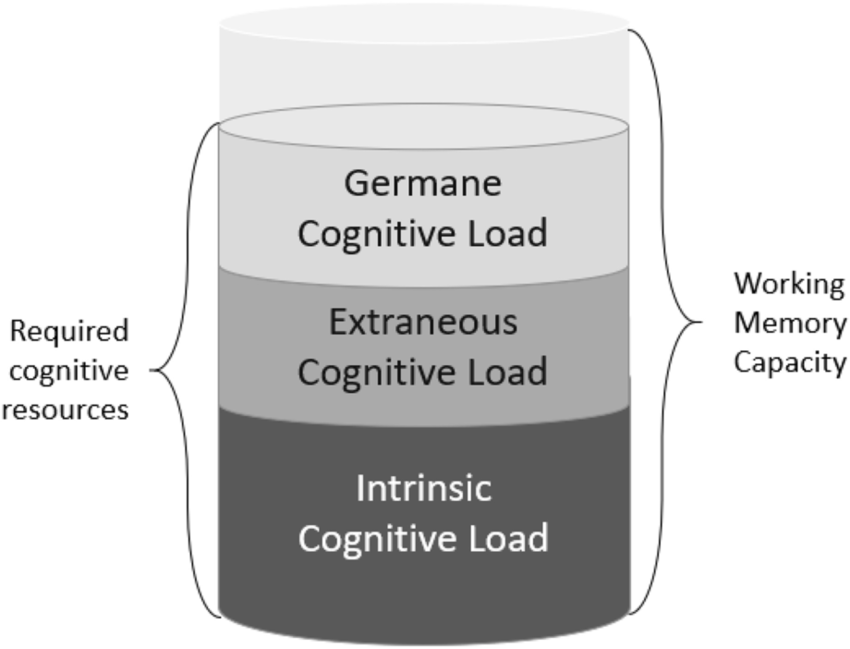
\includegraphics[width=0.75\textwidth]{image/cognitive-load-theory.png}
  \caption{Tiga jenis beban kognitif dalam \textit{Cognitive Load Theory}: \textit{intrinsic}, \textit{extraneous}, dan \textit{germane load} (diadaptasi dari \textcite{sweller1988})}
  \label{fig:cognitive-load}
\end{figure}

\textcite{skulmowski2022} mengembangkan pemahaman CLT dengan mengadaptasinya untuk lingkungan digital dan pembelajaran daring. Penelitian mereka mengusulkan perspektif baru tentang \textit{extraneous cognitive load} yang mempertimbangkan karakteristik unik media digital, seperti konten yang kaya secara perseptual, distraksi visual, dan desain antarmuka yang kompleks. Mereka berargumen bahwa media digital menciptakan bentuk \textit{extraneous load} yang berbeda dari media tradisional, terutama melalui elemen-elemen yang tidak relevan dengan tujuan pembelajaran atau pemrosesan informasi inti. Temuan ini sangat relevan untuk memahami bagaimana antarmuka Telegram yang penuh dengan pesan, emoji, dan media visual dapat meningkatkan beban kognitif ekstrinsik bagi anggota yang mencoba mengekstrak informasi investasi yang relevan.

Penelitian empiris oleh \textcite{sidnammauch2024} menerapkan CLT secara khusus pada konteks distraksi media sosial melalui studi dengan 1.026 partisipan. Mereka mengintegrasikan \textit{load theory of attention} dengan kerangka \textit{uses and gratifications} untuk menjelaskan bagaimana media sosial mobile menciptakan distraksi melalui sumber daya kognitif yang terbatas. Studi mereka mendemonstrasikan bahwa individu dengan kapasitas memori kerja yang lebih rendah lebih rentan terhadap distraksi media sosial, dan bahwa \textit{affordances} teknologi seperti notifikasi \textit{push} dan aksesibilitas konstan memperburuk masalah ini. Temuan ini memperkuat argumen bahwa komunitas Telegram finansial dengan lebih dari 22.000 anggota dan aliran pesan yang konstan menciptakan lingkungan yang sangat rentan terhadap \textit{cognitive overload} dan distraksi, yang pada akhirnya dapat menurunkan kualitas pengambilan keputusan investasi.

\subsection{Ekonomi Perhatian di Media Sosial}

\textcite{heitmayer2025} memberikan perspektif teoretis terbaru dengan mengusulkan bahwa perhatian (\textit{attention}) berfungsi sebagai mata uang simbolis universal di media sosial. Penelitian ini memperkenalkan model \textit{dual-stream} yang membedakan antara perhatian yang "mengalir" (\textit{flow attention}) dan perhatian yang "mengeras" (\textit{calcified attention}). \textit{Flow attention} mengacu pada alokasi perhatian yang dinamis dan sementara terhadap konten yang terus berubah, sementara \textit{calcified attention} merujuk pada investasi perhatian jangka panjang yang termanifestasi dalam bentuk \textit{followers}, \textit{likes}, atau keanggotaan komunitas. Dalam konteks komunitas finansial Telegram, kedua bentuk perhatian ini bersaing: anggota harus mengalokasikan \textit{flow attention} mereka untuk memproses aliran pesan yang konstan, sementara \textit{calcified attention} mereka termanifestasi dalam komitmen berkelanjutan terhadap komunitas dan kepercayaan terhadap sumber informasi tertentu seperti Michael Yeoh. Kelangkaan perhatian (\textit{attention scarcity}) yang diidentifikasi dalam penelitian ini menjadi masalah sentral yang harus diatasi oleh sistem rangkuman otomatis dengan memaksimalkan efisiensi alokasi perhatian anggota.

Analisis empiris oleh \textcite{nematzadeh2019} tentang \textit{information overload} dalam komunikasi grup menggunakan data dari platform Twitch menunjukkan bagaimana peningkatan volume pesan dalam grup dapat menyebabkan transisi dari percakapan yang koheren menjadi "kakofoni" di mana informasi bermakna tenggelam dalam kebisingan. Mereka mengidentifikasi bahwa ketika laju pesan melebihi ambang batas tertentu, kualitas percakapan menurun drastis, partisipasi menjadi tidak merata, dan informasi penting hilang. Fenomena ini sangat relevan dengan komunitas Telegram finansial yang diteliti, di mana pesan dapat muncul dengan laju ratusan per jam selama jam perdagangan aktif. Sistem rangkuman otomatis yang dirancang dalam penelitian ini bertujuan untuk mengatasi transisi menuju kakofoni ini dengan menyaring dan mensintesis informasi kunci secara periodik.


% ==========================================
\section{\textit{Text Summarization} dengan \textit{Large Language Models}}
\label{sec:text-summarization}

Peringkasan teks otomatis telah mengalami evolusi signifikan dengan munculnya model bahasa berbasis \textit{transformer} dan \textit{large language models} (LLMs). Bagian ini mengulas perkembangan metodologi peringkasan teks dari pendekatan berbasis ekstraksi hingga generasi abstraktif dengan LLMs, dengan fokus khusus pada tantangan peringkasan multi-dokumen dan percakapan yang relevan dengan konteks komunitas Telegram.

\subsection{Fondasi: Arsitektur \textit{Transformer} dan BERT}

Sebelum membahas aplikasi model bahasa dalam peringkasan teks, penting untuk memahami arsitektur fundamental yang mendasari perkembangan NLP modern: \textit{Transformer} dan \textit{Bidirectional Encoder Representations from Transformers} (BERT). Kedua inovasi ini telah merevolusi pemrosesan bahasa alami dan menjadi dasar bagi hampir semua model bahasa kontemporer yang digunakan dalam penelitian ini.

\textcite{vaswani2017} memperkenalkan arsitektur \textit{Transformer} yang menggantikan arsitektur rekuren tradisional (\textit{RNN}, \textit{LSTM}) dengan mekanisme \textit{self-attention} yang dapat memproses seluruh urutan input secara paralel. Inovasi kunci dari \textit{Transformer} adalah kemampuannya untuk menangkap dependensi jarak jauh dalam teks tanpa keterbatasan memori yang dialami oleh arsitektur rekuren. Mekanisme \textit{multi-head attention} memungkinkan model untuk menghadiri berbagai aspek representasional input secara simultan, sementara \textit{positional encoding} mempertahankan informasi tentang urutan kata. Arsitektur \textit{encoder-decoder} yang diusulkan terdiri dari tumpukan lapisan \textit{transformer} yang masing-masing mengandung sub-lapisan \textit{multi-head self-attention} dan \textit{feed-forward neural network}. Penelitian seminal ini mencapai hasil \textit{state-of-the-art} pada tugas terjemahan mesin dan menetapkan \textit{Transformer} sebagai arsitektur dominan untuk NLP.

\begin{figure}[H]
  \centering
  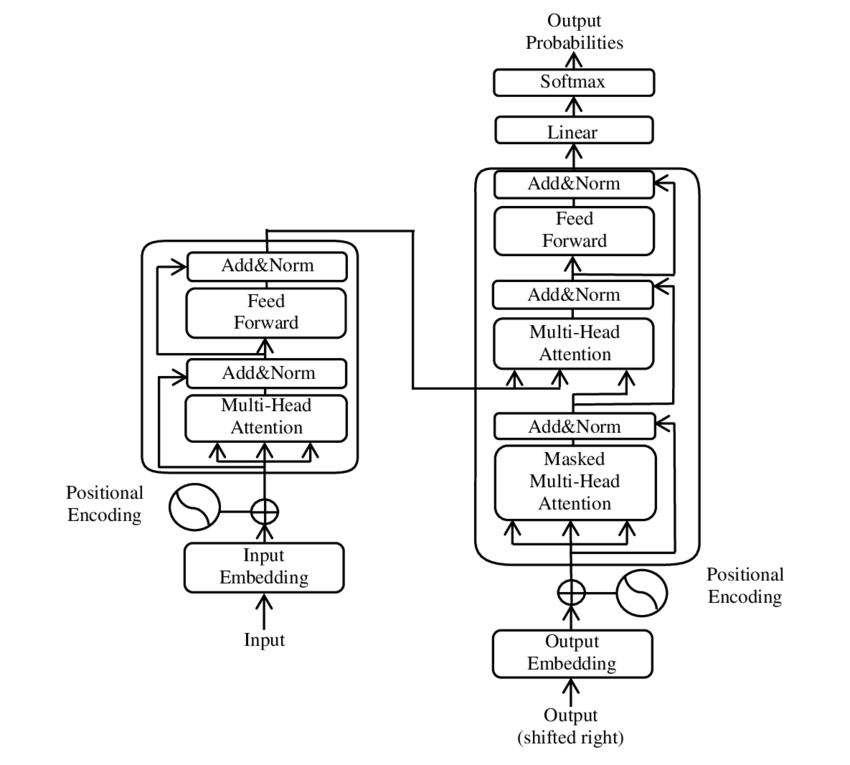
\includegraphics[width=0.65\textwidth]{image/transformer-architecture.png}
  \caption{Arsitektur Transformer dengan mekanisme \textit{multi-head attention} dan struktur \textit{encoder-decoder} (diadaptasi dari \textcite{vaswani2017})}
  \label{fig:transformer-arch}
\end{figure}

\textcite{devlin2019} mengembangkan konsep \textit{Transformer} lebih lanjut dengan memperkenalkan BERT (\textit{Bidirectional Encoder Representations from Transformers}), model bahasa yang dilatih secara \textit{bidirectional} menggunakan arsitektur \textit{Transformer encoder}. Berbeda dengan model bahasa unidirectional sebelumnya yang hanya memproses teks dari kiri ke kanan atau kanan ke kiri, BERT dilatih menggunakan dua tugas pra-latih: \textit{Masked Language Modeling} (MLM), di mana sebagian token input di-\textit{mask} dan model harus memprediksinya berdasarkan konteks bidirectional, dan \textit{Next Sentence Prediction} (NSP), di mana model memprediksi apakah dua kalimat berurutan dalam teks original. Pendekatan \textit{pre-training} dan \textit{fine-tuning} yang diusulkan memungkinkan BERT untuk mencapai performa \textit{state-of-the-art} pada sebelas tugas NLP yang beragam, termasuk klasifikasi teks, \textit{question answering}, dan \textit{natural language inference}. Representasi kontekstual bidirectional yang dihasilkan BERT menangkap nuansa semantik yang tidak dapat ditangkap oleh model unidirectional atau representasi statis seperti Word2Vec.

Gambar \ref{fig:bert-architecture} mengilustrasikan arsitektur BERT dan perbedaannya dengan model bahasa unidirectional. Arsitektur ini menjadi fondasi bagi berbagai varian yang digunakan dalam penelitian ini, termasuk IndoBERT untuk bahasa Indonesia, RoBERTa untuk klasifikasi emosi, dan model NER berbasis BERT untuk ekstraksi entitas finansial.

\begin{figure}[H]
  \centering
  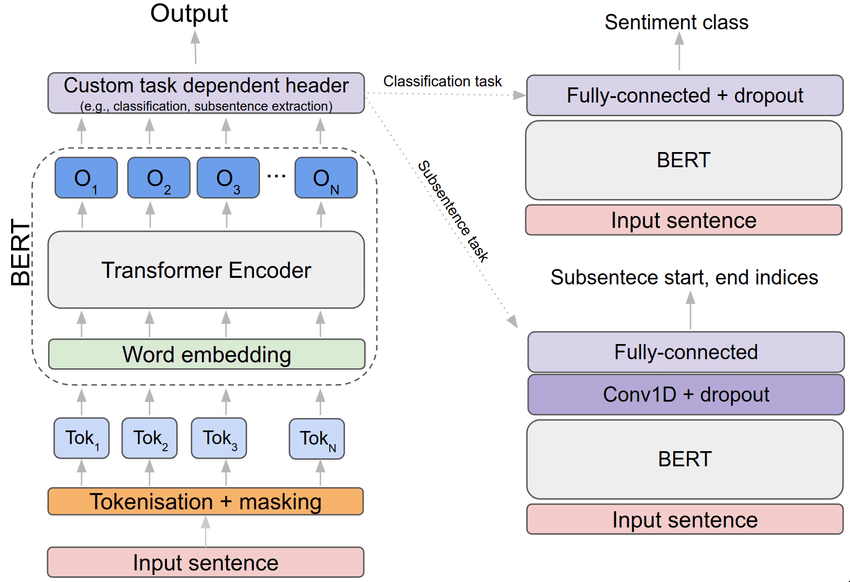
\includegraphics[width=0.85\textwidth]{image/bert-architecture-diagram.png}
  \caption{Arsitektur BERT menunjukkan mekanisme \textit{bidirectional self-attention} dan proses \textit{pre-training} dengan \textit{Masked Language Modeling} (diadaptasi dari \textcite{devlin2019})}
  \label{fig:bert-architecture}
\end{figure}

Kontribusi BERT terhadap NLP tidak hanya terletak pada performa superiornya pada berbagai \textit{benchmark}, tetapi juga pada paradigma \textit{transfer learning} yang efektif: model bahasa umum yang besar dilatih pada korpus teks masif, kemudian di-\textit{fine-tune} untuk tugas spesifik dengan data berlabel yang relatif terbatas. Paradigma ini sangat relevan dengan konteks penelitian ini, di mana model IndoBERT yang telah dilatih pada korpus bahasa Indonesia umum di-\textit{fine-tune} untuk tugas-tugas spesifik domain finansial seperti analisis sentimen dan ekstraksi entitas.

\subsection{Peringkasan Berbasis \textit{Transformer}}

\textcite{liu2019bertsum} memperkenalkan pendekatan \textit{BERTSum} yang memanfaatkan representasi BERT untuk peringkasan ekstraktif dan abstraktif. Penelitian mereka mendemonstrasikan bahwa model \textit{encoder} tingkat dokumen yang dibangun di atas BERT dengan lapisan \textit{Transformer} antar-kalimat dapat menghasilkan rangkuman berkualitas tinggi. Pendekatan dua tahap \textit{fine-tuning} yang mereka usulkan, di mana model pertama-tama di-\textit{fine-tune} untuk tugas ekstraksi kalimat sebelum dilatih untuk generasi abstraktif, menetapkan metodologi dasar yang diadopsi oleh banyak penelitian berikutnya. Kontribusi kunci dari penelitian ini adalah demonstrasi bahwa model bahasa pra-latih dapat secara efektif menangkap struktur dokumen dan hubungan semantik antar-kalimat, yang esensial untuk menghasilkan rangkuman yang koheren dan informatif.

Pemahaman tentang \textit{trade-off} antara peringkasan ekstraktif dan abstraktif diperluas oleh penelitian \textcite{pilault2020}, yang membandingkan kedua pendekatan menggunakan model \textit{transformer} pada dokumen panjang. Evaluasi manusia mereka mengungkapkan temuan penting: sementara pendekatan abstraktif berbasis \textit{transformer} unggul dalam koherensi dan kelancaran, metode ekstraktif cenderung mencetak lebih tinggi dalam hal informativeness. Temuan ini menginformasikan desain sistem dalam penelitian ini, di mana pendekatan hibrida digunakan: BERTopic untuk ekstraksi topik dan entitas kunci (pendekatan ekstraktif), dikombinasikan dengan Llama 3.1 70B untuk generasi rangkuman naratif yang koheren (pendekatan abstraktif).

\begin{figure}[H]
  \centering
  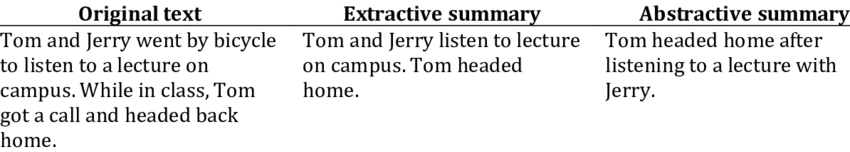
\includegraphics[width=0.8\textwidth]{image/extractive-vs-abstractive.png}
  \caption{Perbandingan pendekatan peringkasan ekstraktif (memilih kalimat penting) dan abstraktif (menghasilkan teks baru) menunjukkan \textit{trade-off} antara \textit{informativeness} dan koherensi}
  \label{fig:extract-abstract}
\end{figure}

\subsection{Peringkasan Multi-Dokumen dan Sintesis Informasi}

Tantangan peringkasan multi-dokumen, yang sangat relevan dengan konteks sintesis lintas tiga grup Telegram, dibahas secara komprehensif oleh \textcite{deyoung2024}. Penelitian mereka mengajukan pertanyaan fundamental: apakah model peringkasan multi-dokumen modern benar-benar dapat mensintesis informasi, atau hanya melakukan agregasi sederhana? Melalui evaluasi terhadap berbagai model dari \textit{fine-tuned transformers} hingga GPT-4, mereka menemukan bahwa sebagian besar model mengalami kesulitan dalam mensintesis informasi yang bertentangan atau berbeda perspektif, dan sangat sensitif terhadap urutan input dokumen. Temuan kritis ini memiliki implikasi langsung bagi desain sistem dalam penelitian ini: sistem harus dirancang dengan mekanisme eksplisit untuk menangani informasi yang mungkin bertentangan antara grup "Cuap Cuap", "Swing Plan", dan "Advanced Group", dan tidak boleh bergantung semata-mata pada kemampuan sintesis implisit LLM.

\textcite{ravaut2024} menyediakan wawasan penting tentang bagaimana LLMs memanfaatkan konteks panjang dalam peringkasan. Penelitian mereka mengungkapkan masalah \textit{position bias}, di mana LLMs cenderung memberikan bobot yang tidak merata terhadap informasi berdasarkan posisinya dalam konteks. Mereka mengevaluasi enam LLMs berbeda pada sepuluh dataset dengan lima metrik evaluasi, menemukan bahwa model cenderung memberikan perhatian berlebihan pada informasi di awal dan akhir konteks, sementara mengabaikan informasi di tengah. Untuk mengatasi masalah ini, mereka memperkenalkan benchmark \textit{MiddleSum} dan mengevaluasi metode hierarkis dan inkremental untuk peringkasan. Temuan ini sangat relevan untuk implementasi Llama 3.1 70B dalam penelitian ini, yang harus memproses konteks panjang (potensial ratusan pesan dalam satu jam). Desain sistem harus mempertimbangkan strategi mitigasi \textit{position bias}, seperti pengelompokan pesan berdasarkan topik sebelum peringkasan atau penggunaan rangkuman inkremental.

\subsection{Peringkasan Percakapan dan Dialog}

\textcite{gliwa2019} memperkenalkan \textit{SAMSum Corpus}, dataset dialog yang dianotasi secara manual untuk peringkasan abstraktif, yang menetapkan bahwa peringkasan percakapan memiliki tantangan unik dibandingkan dengan peringkasan artikel berita. Dialog dan percakapan grup memiliki struktur yang lebih kompleks dengan pergantian pembicara, konteks implisit, referensi anaforik, dan topik yang bercabang. Dataset mereka mendemonstrasikan pentingnya memahami struktur dialog dan dinamika percakapan untuk menghasilkan rangkuman yang akurat dan informatif. Karakteristik ini sangat relevan dengan konteks Telegram, di mana percakapan dapat melibatkan puluhan pembicara dengan topik yang berubah cepat dan sering kali tumpang tindih.

\textcite{tian2024} mengembangkan metodologi peringkasan dialog lebih lanjut dengan mengusulkan pendekatan \textit{Mixture of Experts} (MoE) berbasis LLM. Penelitian mereka memperkenalkan mekanisme \textit{role-oriented routing} yang memilih model atau strategi peringkasan yang sesuai berdasarkan karakteristik informasi percakapan yang berbeda. Pendekatan ini sangat relevan dengan konteks komunitas finansial Telegram yang berjenjang, di mana pesan dari berbagai peran (misalnya, Michael Yeoh sebagai pemimpin komunitas versus anggota biasa) mungkin memerlukan perlakuan berbeda dalam proses peringkasan. Sistem yang dirancang dalam penelitian ini mengadopsi konsep serupa melalui \textit{weighted sentiment analysis} yang memberikan bobot berbeda berdasarkan peran pengirim pesan.

\subsection{Memori Jangka Panjang dalam Sistem Dialog}

Konsep memori jangka panjang dalam sistem percakapan dieksplorasi oleh \textcite{wang2023recursive}, yang mengusulkan metode peringkasan rekursif untuk memungkinkan LLMs mempertahankan konteks percakapan yang panjang. Pendekatan mereka melibatkan pembuatan rangkuman hierarkis dari konteks dialog yang kemudian digunakan untuk menjaga konsistensi dalam percakapan yang berkepanjangan. Konsep ini paralel dengan desain sistem rangkuman per jam dalam penelitian ini, di mana setiap rangkuman per jam dapat dipandang sebagai pembentukan "memori jangka panjang" bagi komunitas. Akumulasi rangkuman per jam ini dapat membentuk representasi terkompresi dari diskusi komunitas yang memungkinkan anggota untuk memahami tren dan perkembangan informasi tanpa harus membaca setiap pesan individual.

\subsection{Metrik Evaluasi untuk Peringkasan}

Evaluasi kualitas rangkuman otomatis merupakan aspek kritis yang dibahas oleh \textcite{zhang2020bertscore}. Mereka memperkenalkan \textit{BERTScore}, metrik evaluasi yang menggunakan \textit{contextual embeddings} dari BERT untuk menghitung kesamaan antara rangkuman yang dihasilkan dan rangkuman referensi, mengatasi keterbatasan metrik berbasis \textit{n-gram} seperti ROUGE yang hanya menghitung kecocokan kata eksak. \textit{BERTScore} mendemonstrasikan korelasi yang lebih baik dengan penilaian manusia karena dapat mengenali parafrase dan kesamaan semantik yang tidak tertangkap oleh metrik tradisional. Penelitian ini mengadopsi \textit{BERTScore} bersama dengan metrik lain untuk evaluasi komprehensif kualitas rangkuman yang dihasilkan sistem.

Namun, \textcite{shen2023} memberikan peringatan penting tentang penggunaan LLMs sebagai evaluator otomatis untuk peringkasan abstraktif. Melalui analisis ekstensif terhadap ChatGPT dan GPT-4 sebagai evaluator, mereka menemukan masalah signifikan dalam stabilitas, reliabilitas, dan ketergantungan pada dimensi evaluasi tertentu. Temuan mereka menunjukkan bahwa evaluasi otomatis berbasis LLM tidak dapat sepenuhnya menggantikan evaluasi manusia, terutama untuk aspek kualitatif seperti koherensi naratif dan relevansi kontekstual. Implikasi bagi penelitian ini adalah perlunya kombinasi antara metrik otomatis (\textit{BERTScore}, ROUGE) dan evaluasi subjektif melalui \textit{feedback} pengguna komunitas untuk mendapatkan penilaian holistik terhadap kualitas rangkuman.

% ==========================================
\section{Analisis Sentimen untuk Media Sosial Finansial}
\label{sec:sentiment-analysis}

Analisis sentimen merupakan komponen esensial dalam memahami dinamika diskusi finansial di media sosial. Bagian ini mengulas perkembangan metodologi analisis sentimen, dengan fokus khusus pada domain finansial dan pemrosesan bahasa Indonesia, serta mengeksplorasi bagaimana sinyal sentimen dari komunitas dapat dimanfaatkan untuk meningkatkan kualitas rangkuman.

\subsection{Model Bahasa untuk Analisis Sentimen Indonesia}

\textcite{wilie2020} memperkenalkan \textit{IndoNLU}, benchmark komprehensif untuk evaluasi pemahaman bahasa Indonesia yang mencakup dua belas tugas termasuk analisis sentimen. Dataset mereka dilatih pada \textit{Indo4B}, korpus bahasa Indonesia dengan empat miliar kata, dan menyediakan model IndoBERT yang mengungguli \textit{multilingual BERT} (mBERT) pada berbagai tugas. Penelitian ini mendemonstrasikan bahwa model bahasa monolingual yang dilatih khusus pada korpus bahasa Indonesia menghasilkan performa superior dibandingkan model multilingual untuk tugas-tugas NLP Indonesia. Kontribusi mereka menetapkan IndoBERT sebagai baseline untuk berbagai aplikasi NLP Indonesia, termasuk implementasi analisis sentimen dalam penelitian ini yang menggunakan \textit{indonesian-roberta-base-emotion-classifier}.

Penelitian oleh \textcite{koto2020} memperkuat temuan ini dengan memperkenalkan \textit{IndoLEM}, benchmark dataset dan model IndoBERT untuk NLP Indonesia. Mereka mendemonstrasikan bahwa \textit{pre-training} pada korpus bahasa Indonesia yang besar (220 juta kata) menghasilkan representasi bahasa yang lebih baik untuk tugas-tugas \textit{downstream} termasuk analisis sentimen, yang mencapai F1-score 84,13\%. Penelitian mereka juga mengeksplorasi \textit{transfer learning} dari model multibahasa, menunjukkan bahwa meskipun model multibahasa dapat memberikan titik awal yang baik, \textit{fine-tuning} pada data Indonesia sangat meningkatkan performa.

\textcite{nugroho2021} menerapkan \textit{fine-tuning} BERT untuk analisis sentimen pada ulasan aplikasi mobile berbahasa Indonesia, konteks yang memiliki kesamaan dengan teks media sosial karena sifatnya yang informal dan sering mengandung bahasa gaul atau singkatan. Penelitian mereka membandingkan model multibahasa dengan model khusus Indonesia, mendemonstrasikan keunggulan \textit{transfer learning} untuk bahasa Indonesia dengan data berlabel terbatas. Temuan mereka sangat relevan dengan penelitian ini, karena pesan Telegram finansial sering kali menggunakan bahasa informal, singkatan, dan istilah khusus yang memerlukan model yang robust terhadap variasi linguistik.

\subsection{Analisis Sentimen Domain Finansial}

\textcite{araci2019} memperkenalkan \textit{FinBERT}, model BERT pertama yang dilatih khusus pada korpus finansial untuk analisis sentimen. Model ini mencapai peningkatan akurasi 15\% dibandingkan BERT umum pada dataset \textit{Financial PhraseBank} dan FiQA. Penelitian ini mendemonstrasikan pentingnya \textit{domain-specific pre-training} untuk teks finansial, yang memiliki karakteristik linguistik unik termasuk terminologi khusus, struktur kalimat formal, dan nuansa sentimen yang berbeda dari domain umum. Konsep sentimen dalam konteks finansial lebih kompleks daripada klasifikasi positif-negatif sederhana; istilah seperti "volatilitas tinggi" dapat memiliki konotasi positif atau negatif tergantung konteks strategi investasi. Temuan ini memotivasi penggunaan model analisis sentimen yang disesuaikan untuk konteks finansial dalam penelitian ini, meskipun disesuaikan untuk bahasa Indonesia.

\textcite{si2014} mengeksplorasi pemanfaatan sentimen media sosial untuk prediksi pergerakan saham dengan mengintegrasikan analisis sentimen Twitter dengan struktur relasi sosial. Penelitian mereka mendemonstrasikan bahwa menggabungkan sentimen dengan informasi jaringan sosial (siapa yang mempengaruhi siapa) secara signifikan meningkatkan akurasi prediksi pergerakan harga saham. Temuan kunci mereka adalah bahwa tidak semua opini memiliki bobot yang sama; pendapat dari individu yang lebih berpengaruh atau kredibel dalam jaringan sosial harus diberi bobot lebih tinggi. Konsep ini memiliki paralel langsung dengan desain sistem dalam penelitian ini, di mana implementasi \textit{weighted sentiment analysis} memberikan bobot berbeda berdasarkan peran pengirim (Michael Yeoh versus anggota biasa), mengakui bahwa tidak semua kontributor dalam komunitas memiliki tingkat pengaruh atau keahlian yang sama.

\subsection{Pemanfaatan Sinyal Komunitas dalam Peringkasan}

\textcite{kano2018} mengusulkan metodologi inovatif untuk memanfaatkan sinyal popularitas dalam media sosial (seperti \textit{votes}, \textit{shares}, \textit{bookmarks}) sebagai label jarak jauh (\textit{distant labels}) untuk peringkasan ekstraktif percakapan online. Penelitian mereka mendemonstrasikan bahwa metrik keterlibatan komunitas dapat berfungsi sebagai indikator kualitas dan relevansi konten, memisahkan kontribusi konten dari faktor kontekstual. Pendekatan ini sangat relevan dengan konteks komunitas Telegram finansial berjenjang dalam penelitian ini, di mana struktur hierarkis (grup "Cuap Cuap", "Swing Plan", "Advanced Group") dan peran pengguna (pemimpin komunitas versus anggota biasa) dapat dimanfaatkan sebagai sinyal implisit tentang pentingnya informasi. Prinsip pemanfaatan sinyal komunitas ini diadopsi secara langsung dalam penelitian ini, di mana "peran pengguna" (misalnya, admin Michael Yeoh versus anggota biasa) digunakan sebagai proksi untuk "popularitas" atau "kredibilitas" informasi, yang kemudian menjadi dasar bagi fitur \textit{weighted sentiment}. Sistem yang dikembangkan mengimplementasikan \textit{weighted sentiment} yang memberikan bobot lebih tinggi pada pesan dari sumber yang lebih kredibel atau berpengaruh dalam komunitas.

\subsection{Klasifikasi Emosi versus Sentimen untuk Investor Ritel}

Pemilihan \textit{indonesian-roberta-base-emotion-classifier} dalam penelitian ini memerlukan justifikasi teoretis, karena berbeda dari pendekatan analisis sentimen finansial konvensional yang fokus pada klasifikasi bullish/bearish atau positif/negatif. Perbedaan fundamental ini didasarkan pada karakteristik unik investor ritel dibandingkan dengan investor institusional atau analis profesional.

Penelitian perilaku keuangan menunjukkan bahwa keputusan investasi ritel sangat dipengaruhi oleh emosi, terutama ketakutan (\textit{fear}) dan keserakahan (\textit{greed}). Berbeda dengan analis profesional yang dilatih untuk membuat keputusan berdasarkan analisis rasional, investor ritel sering kali membuat keputusan yang didorong oleh reaksi emosional terhadap pergerakan pasar atau diskusi komunitas. Dalam konteks komunitas Telegram dengan lebih dari 22.000 anggota yang sebagian besar adalah investor ritel muda, emosi kolektif yang terekspresikan dalam diskusi dapat berfungsi sebagai indikator sentimen pasar yang lebih akurat daripada sekadar klasifikasi positif/negatif.

Model klasifikasi emosi yang digunakan dalam penelitian ini dapat mendeteksi spektrum emosi yang lebih nuansa, termasuk ketakutan, kegembiraan, kemarahan, dan kesedihan. Emosi-emosi ini memberikan sinyal yang lebih kaya tentang psikologi pasar dibandingkan dengan sentimen biner. Misalnya, ekspresi ketakutan tinggi dalam diskusi komunitas dapat mengindikasikan potensi \textit{panic selling}, sementara kegembiraan berlebihan dapat menandakan \textit{euphoria} yang sering kali mendahului koreksi pasar. Pendekatan berbasis emosi ini selaras dengan teori \textit{behavioral finance} yang mengidentifikasi bias psikologis sebagai faktor kunci dalam pengambilan keputusan investasi ritel.

Lebih lanjut, konteks diskusi informal di Telegram lebih cenderung mengekspresikan emosi autentik dibandingkan dengan laporan finansial formal atau analisis profesional. Anggota komunitas sering kali berbagi reaksi emosional mereka terhadap pergerakan harga, keputusan investasi, atau berita pasar dengan cara yang langsung dan tidak tersaring. Klasifikasi emosi dapat menangkap sinyal-sinyal psikologis ini yang hilang dalam analisis sentimen tradisional, memberikan wawasan yang lebih mendalam tentang suasana hati (\textit{mood}) komunitas dan potensi implikasinya terhadap perilaku investasi kolektif.

\begin{figure}[H]
  \centering
  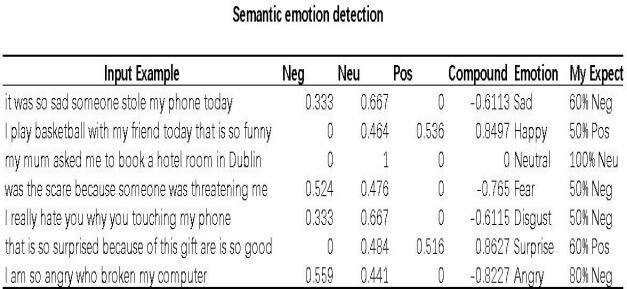
\includegraphics[width=0.75\textwidth]{image/sentiment-analysis-example.jpg}
  \caption{Contoh klasifikasi emosi pada teks menggunakan model \textit{semantic emotion detection}, menunjukkan deteksi berbagai emosi seperti \textit{sad}, \textit{happy}, \textit{fear}, \textit{disgust}, \textit{surprise}, dan \textit{angry} beserta skor probabilitasnya}
  \label{fig:sentiment-example}
\end{figure}

% ==========================================
\section{\textit{Named Entity Recognition} untuk Teks Finansial Indonesia}
\label{sec:ner}

\textit{Named Entity Recognition} (NER) merupakan tugas fundamental dalam NLP yang bertujuan mengidentifikasi dan mengklasifikasikan entitas bernama dalam teks, seperti nama orang, organisasi, lokasi, dan dalam konteks finansial, nama perusahaan, kode saham (ticker), dan istilah finansial spesifik. Berbeda dengan Section \ref{sec:sentiment-analysis} yang fokus pada ekstraksi sinyal sentimen (\textit{apa yang dirasakan}), NER berfokus pada identifikasi entitas (\textit{siapa} atau \textit{apa yang dibahas}). Kedua komponen ini bersifat komplementer dalam sistem rangkuman: NER mengidentifikasi saham mana yang dibahas, sementara analisis sentimen mengidentifikasi bagaimana komunitas merasakan saham tersebut.

\subsection{NER untuk Bahasa Indonesia}

Sebagaimana telah dibahas dalam Section \ref{sec:sentiment-analysis}, model IndoBERT dari \textcite{koto2020} telah menetapkan fondasi kuat untuk berbagai tugas NLP Indonesia, termasuk NER. Dataset \textit{IndoLEM} yang mereka kembangkan menyediakan benchmark NER bahasa Indonesia yang komprehensif, di mana IndoBERT mencapai performa \textit{state-of-the-art} dengan mengungguli mBERT secara signifikan. Model \textit{cahya/bert-base-indonesian-NER} yang digunakan dalam penelitian ini dibangun di atas arsitektur IndoBERT ini, yang telah di-\textit{fine-tune} khusus untuk tugas ekstraksi entitas.

Penelitian \textcite{khairunnisa2020} mengidentifikasi masalah kritis dalam dataset NER Indonesia yang ada: inkonsistensi anotasi yang dapat menurunkan performa model. Mereka menyediakan dataset yang dianotasi ulang dengan standar yang lebih konsisten dan mengevaluasi berbagai pendekatan \textit{deep learning} termasuk BiLSTM-CRF dengan berbagai jenis \textit{embeddings}. Penelitian mereka menekankan pentingnya kualitas data pelatihan dan konsistensi skema anotasi untuk mencapai performa NER yang optimal. Wawasan ini relevan dengan penelitian ini, terutama dalam konteks adaptasi model NER untuk mengenali entitas finansial spesifik Indonesia yang mungkin tidak terwakili dengan baik dalam dataset NER umum, termasuk penggunaan \textit{whitelist} ticker saham dari Bursa Efek Indonesia untuk meningkatkan akurasi deteksi.

\begin{figure}[H]
  \centering
  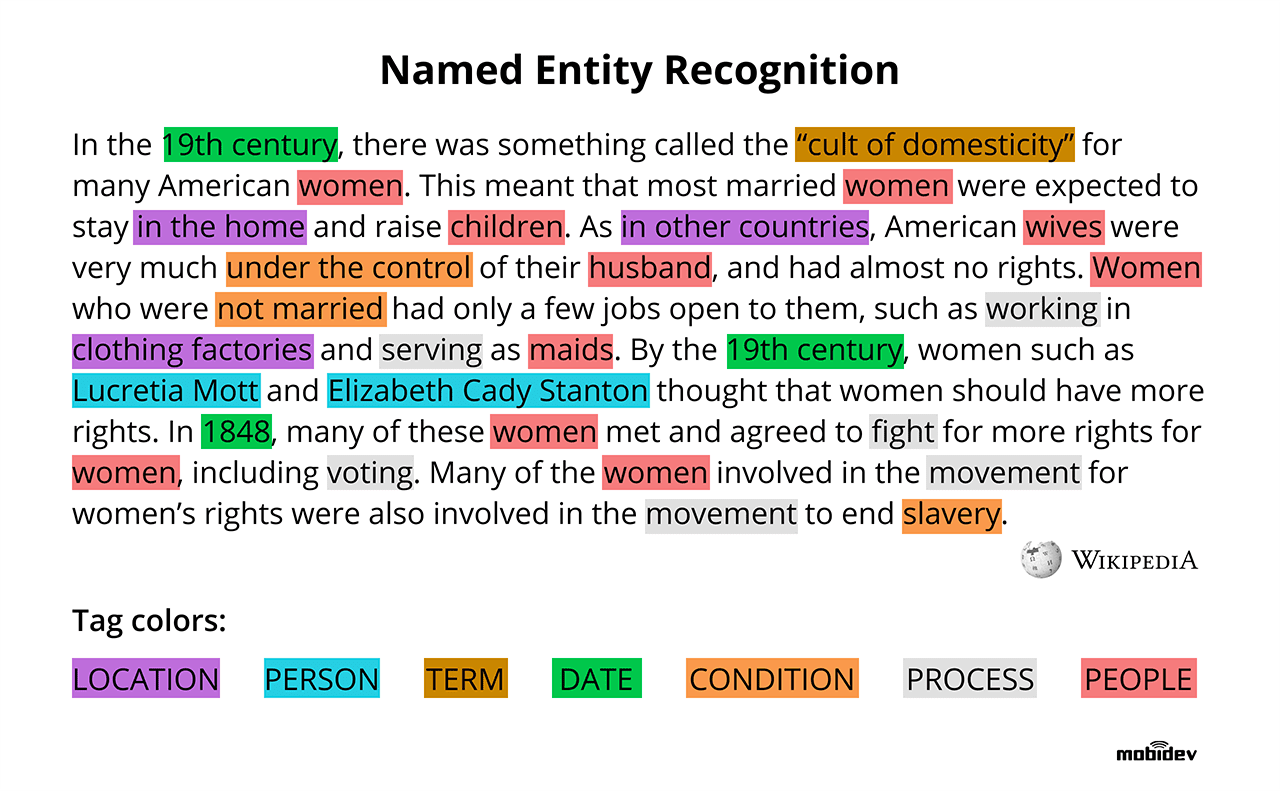
\includegraphics[width=0.85\textwidth]{image/ner-example.png}
  \caption{Contoh \textit{Named Entity Recognition} pada teks, menunjukkan identifikasi berbagai jenis entitas seperti nama orang (\textit{PERSON}), lokasi (\textit{LOCATION}), tanggal (\textit{DATE}), dan istilah khusus (\textit{TERM}) yang diberikan label dan warna berbeda}
  \label{fig:ner-example}
\end{figure}

\subsection{NER Domain Finansial}

\textcite{zhang2022finbert} mengembangkan \textit{FinBERT-MRC}, pendekatan NER finansial yang merumuskan tugas ekstraksi entitas sebagai masalah \textit{machine reading comprehension}. Model mereka mencapai F1-score 92,78\% dan 96,80\% pada dataset finansial Tiongkok, mengungguli pendekatan BiLSTM-CRF dan BERT-CRF tradisional. Penelitian ini mendemonstrasikan bahwa NER domain finansial memiliki tantangan unik karena variasi semantik dan leksikal yang spesifik, seperti perbedaan antara nama perusahaan dalam konteks berita versus dokumen formal, atau ambiguitas antara nama organisasi dan produk finansial. Meskipun penelitian mereka fokus pada bahasa Tiongkok, prinsip-prinsip metodologis dapat diadaptasi untuk konteks Indonesia, terutama dalam menangani ambiguitas nama perusahaan versus kode saham.

\textcite{shah2023} menyediakan sumber daya penting untuk NER finansial melalui \textit{FiNER-ORD}, dataset NER finansial \textit{open research} pertama dengan kualitas tinggi. Dataset ini mengatasi variasi semantik dan leksikal yang unik dalam domain finansial dan menyediakan benchmark untuk berbagai model bahasa pra-latih termasuk varian BERT dan LLMs. Penelitian mereka menekankan bahwa entitas finansial sering kali memiliki representasi multipel (misalnya, "Apple Inc.", "Apple", "AAPL") yang harus dikenali sebagai entitas yang sama. Wawasan ini sangat relevan dengan konteks pasar saham Indonesia, di mana perusahaan mungkin dirujuk dengan nama lengkap, nama singkat, atau kode ticker (misalnya, "Bank Central Asia", "BCA", "BBCA").

% ==========================================
\section{\textit{Topic Modeling} dengan BERTopic}
\label{sec:topic-modeling}

\textit{Topic modeling} merupakan teknik untuk mengidentifikasi tema atau topik abstrak dalam kumpulan dokumen. Bagian ini mengulas evolusi metodologi \textit{topic modeling} dari pendekatan statistik tradisional ke pendekatan berbasis \textit{neural embeddings}, dengan fokus khusus pada BERTopic yang digunakan dalam sistem yang dikembangkan.

\subsection{BERTopic: Metodologi dan Keunggulan}

\textcite{grootendorst2022} memperkenalkan BERTopic, metodologi \textit{topic modeling} neural yang menggabungkan model bahasa berbasis \textit{transformer} (BERT), \textit{document embeddings}, \textit{clustering} dengan HDBSCAN, dan prosedur \textit{class-based TF-IDF} (c-TF-IDF) untuk mengekstrak representasi topik yang koheren. Arsitektur BERTopic mengatasi keterbatasan pendekatan tradisional seperti \textit{Latent Dirichlet Allocation} (LDA) dengan memanfaatkan representasi semantik kontekstual dari \textit{transformer models}. Prosedur c-TF-IDF yang diusulkan menghasilkan representasi topik yang lebih interpretatif dibandingkan dengan metode konvensional dengan memperlakukan semua dokumen dalam satu kluster sebagai satu dokumen besar dan membandingkannya dengan dokumen dari kluster lain. Metodologi ini sangat sesuai untuk teks media sosial yang pendek dan informal, karena tidak memerlukan asumsi distribusional yang ketat seperti LDA.

\begin{figure}[H]
  \centering
  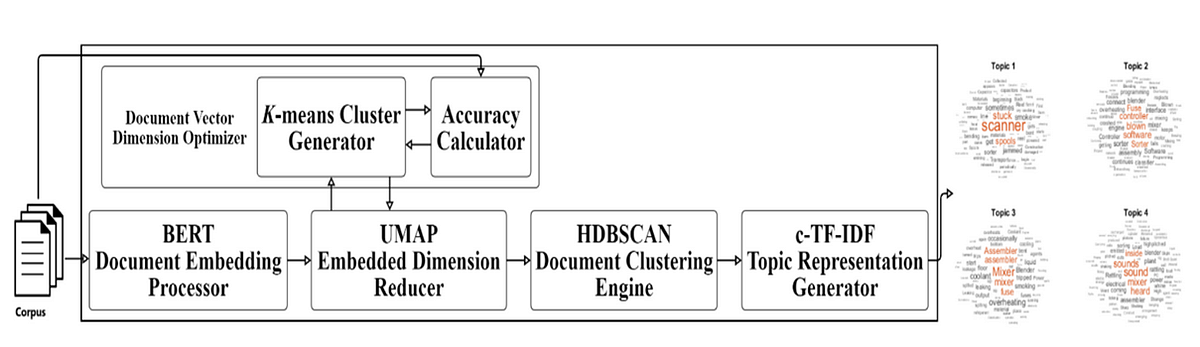
\includegraphics[width=0.85\textwidth]{image/bertopic-workflow.png}
  \caption{Alur kerja BERTopic menunjukkan tahapan dari \textit{document embeddings}, dimensionality reduction dengan UMAP, \textit{clustering} dengan HDBSCAN, hingga ekstraksi representasi topik dengan c-TF-IDF (diadaptasi dari \textcite{grootendorst2022})}
  \label{fig:bertopic-workflow}
\end{figure}

Keunggulan BERTopic untuk teks media sosial divalidasi secara empiris oleh \textcite{egger2022}, yang membandingkan BERTopic dengan LDA, NMF, dan Top2Vec pada dataset 31.800 \textit{tweet} terkait COVID-19 dan perjalanan. Evaluasi mereka mendemonstrasikan superioritas BERTopic untuk teks pendek dan tidak terstruktur, khususnya dalam hal koherensi topik dan interpretabilitas. Metrik evaluasi menunjukkan bahwa BERTopic menghasilkan topik yang lebih koheren dan mudah dipahami dibandingkan dengan metode tradisional, terutama untuk data yang memiliki karakteristik serupa dengan media sosial: panjang dokumen pendek, penggunaan bahasa informal, dan struktur gramatikal yang longgar. Temuan ini memberikan justifikasi kuat untuk pemilihan BERTopic dalam penelitian ini, mengingat pesan Telegram finansial memiliki karakteristik yang sangat mirip dengan \textit{tweet}: pendek, informal, dan sering menggunakan singkatan atau jargon.

\subsection{Perkembangan Terkini dalam \textit{Topic Modeling} Neural}

\textcite{angelov2024} mengembangkan metodologi \textit{topic modeling} lebih lanjut dengan memperkenalkan \textit{Contextual-Top2Vec}, yang menggunakan \textit{contextual token embeddings} dari dokumen untuk menghasilkan topik hierarkis, \textit{topic spans} dalam dokumen, dan label topik berbasis frasa. Penelitian mereka mengusulkan penggunaan \textit{BERTScore} untuk mengevaluasi koherensi dan informativeness topik, mengatasi keterbatasan metrik evaluasi tradisional seperti koherensi berbasis PMI. Model mereka mengungguli pendekatan \textit{state-of-the-art} pada metrik evaluasi komprehensif, mendemonstrasikan bahwa representasi kontekstual dapat meningkatkan kualitas topik yang dihasilkan. Meskipun penelitian ini menggunakan BERTopic sebagai metodologi dasar, wawasan dari \textit{Contextual-Top2Vec} menginformasikan pertimbangan desain, terutama dalam hal evaluasi kualitas topik dan interpretasi hasil \textit{clustering}.

% ==========================================
\section{Telegram sebagai Platform Komunitas}
\label{sec:telegram-platform}

Telegram telah berkembang menjadi platform komunikasi yang dominan untuk komunitas online, terutama di Indonesia. Bagian ini mengulas karakteristik unik Telegram sebagai platform untuk komunitas berskala besar, pola komunikasi yang terjadi di dalamnya, dan implikasi untuk desain sistem analitik dan rangkuman otomatis.

\subsection{Karakteristik dan Dinamika Platform Telegram}

\textcite{nobari2017} menyediakan analisis pionir tentang struktur dan aspek topikal Telegram menggunakan data yang di-\textit{crawl} dari kanal publik. Penelitian mereka mengeksplorasi pola jaringan, klasifikasi pesan (spam/ham), dan arsitektur Telegram sebagai platform \textit{messaging} hibrida yang menggabungkan fitur komunikasi pribadi dan publik. Mereka mengidentifikasi bahwa Telegram memiliki karakteristik unik dibandingkan platform media sosial lain: kombinasi antara privasi komunikasi satu-satu dengan kemampuan penyebaran informasi massal melalui kanal dan grup besar. Struktur ini menciptakan dinamika komunikasi yang berbeda dari platform seperti Twitter atau Facebook, di mana informasi dapat menyebar dengan cepat dalam komunitas tertutup yang besar tanpa eksposur publik yang luas. Pemahaman tentang arsitektur ini penting untuk desain sistem rangkuman yang harus mempertimbangkan privasi komunitas sambil memfasilitasi akses informasi yang efisien.

\textcite{hashemi2019} mengembangkan metodologi untuk mengukur kualitas grup Telegram melalui analisis perilaku pengguna, mengeksplorasi lebih dari 900.000 kanal dan 300.000 \textit{supergroup} berbahasa Persia. Mereka mengusulkan fitur-fitur pengukuran kualitas yang membedakan grup berkualitas tinggi dari grup berkualitas rendah berdasarkan pola aktivitas pengguna, konsistensi partisipasi, dan struktur komunikasi. Penelitian mereka menunjukkan bahwa grup berkualitas tinggi cenderung memiliki partisipasi yang lebih seimbang, topik diskusi yang lebih fokus, dan tingkat spam yang lebih rendah. Temuan ini relevan dengan konteks komunitas Michael Yeoh yang memiliki struktur berjenjang, di mana grup "Advanced" diasumsikan memiliki kualitas diskusi yang lebih tinggi dibandingkan grup "Cuap Cuap" umum. Sistem rangkuman harus dirancang dengan mempertimbangkan perbedaan kualitas dan karakteristik diskusi antar grup.

\subsection{Analisis Skala Besar Komunitas Telegram}

\textcite{lamorgia2024} menyediakan dataset Telegram terbesar hingga saat ini dengan 120.979 kanal dan lebih dari 400 juta pesan, bersama dengan infrastruktur untuk pengumpulan dan analisis data skala besar. Penelitian mereka menyediakan alat dan metodologi untuk penelitian komunitas Telegram yang mencakup analisis dinamika komunitas, propagasi konten, dan pola komunikasi tingkat platform. Kontribusi mereka mendemonstrasikan bahwa Telegram telah berkembang menjadi ekosistem informasi yang kompleks dengan dinamika komunitas yang beragam. Skala dataset ini memberikan konteks untuk memahami bahwa komunitas finansial dengan 22.000+ anggota seperti yang diteliti dalam penelitian ini merupakan bagian dari fenomena komunikasi online yang lebih luas, di mana platform seperti Telegram telah menjadi infrastruktur kritis untuk pertukaran informasi dalam komunitas tematik berskala besar.

Penelitian terbaru oleh \textcite{perlo2025} menyediakan analisis per-topik pertama dari grup Telegram, mengeksplorasi 51 juta pesan dari 669 grup di berbagai topik termasuk Pendidikan, Politik, dan Cryptocurrency. Penelitian mereka menganalisis pola aktivitas pengguna, kehadiran bot, dan berbagi media, serta menyediakan alat \textit{open-source} untuk pengumpulan pesan otomatis. Temuan kunci mereka adalah bahwa grup dengan topik berbeda menunjukkan pola komunikasi yang sangat berbeda dalam hal volume pesan, distribusi waktu aktivitas, dan tipe konten yang dibagikan. Khususnya untuk kategori Cryptocurrency, yang memiliki kesamaan dengan komunitas finansial yang diteliti, mereka menemukan tingkat aktivitas yang sangat tinggi dengan puncak aktivitas yang berkorelasi dengan jam perdagangan pasar. Temuan ini memvalidasi desain sistem rangkuman per jam dalam penelitian ini, karena pola aktivitas temporal yang kuat mengindikasikan bahwa rangkuman periodik sesuai dengan ritme alami diskusi komunitas.

% ==========================================
\section{Arsitektur Pemrosesan Data \textit{Real-Time}}
\label{sec:realtime-architecture}

Implementasi sistem rangkuman otomatis untuk komunitas Telegram yang aktif memerlukan arsitektur pemrosesan data yang dapat menangani aliran pesan secara \textit{real-time} atau \textit{near-real-time}. Bagian ini mengulas pendekatan arsitektural untuk pemrosesan \textit{stream} teks dengan NLP, pola \textit{event-driven architecture}, dan pertimbangan desain untuk sistem yang responsif dan \textit{scalable}.

\subsection{\textit{Pipeline} NLP untuk Pemrosesan \textit{Stream} Teks}

\textcite{hamidi2021} mengusulkan arsitektur \textit{pipeline} NLP yang dinamis dan terdistribusi untuk pemrosesan \textit{stream} teks \textit{real-time}. Penelitian mereka menggunakan Apache Storm dan Apache Kafka untuk menerapkan tugas-tugas NLP pada aliran data tekstual, memungkinkan pengembang untuk menginjeksi modul NLP melalui berbagai bahasa pemrograman dan mendukung sumber data multipel. Arsitektur mereka mendemonstrasikan bagaimana komponen NLP yang berbeda (tokenisasi, \textit{part-of-speech tagging}, \textit{named entity recognition}, analisis sentimen) dapat dikomposisikan dalam \textit{pipeline} yang dapat di-\textit{scale} secara horizontal. Prinsip-prinsip desain ini relevan dengan penelitian ini, di mana sistem harus mengintegrasikan beberapa komponen NLP (analisis sentimen, NER, \textit{topic modeling}, generasi rangkuman) dalam arsitektur yang koheren dan dapat diperluas.

\textcite{isah2019} menyediakan survei komprehensif tentang \textit{framework} pemrosesan \textit{stream} data terdistribusi, termasuk Apache Storm, Spark Streaming, Apache Flink, dan Kafka Streams. Penelitian mereka membandingkan model pemrosesan, karakteristik operasional, dan pola arsitektural dari berbagai \textit{framework}, memberikan taksonomi yang membantu dalam pemilihan teknologi yang sesuai untuk kasus penggunaan spesifik. Untuk konteks komunitas Telegram dengan volume pesan yang tinggi namun tidak ekstrem (ratusan hingga ribuan pesan per jam), mereka mengidentifikasi bahwa pendekatan \textit{micro-batch processing} dengan Kafka atau arsitektur berbasis \textit{event} yang lebih sederhana dapat memberikan keseimbangan optimal antara latensi, throughput, dan kompleksitas implementasi. Wawasan ini menginformasikan desain sistem dalam penelitian ini, yang mengadopsi arsitektur berbasis \textit{event} dengan penjadwalan periodik daripada pemrosesan \textit{stream} kontinu, sesuai dengan kebutuhan rangkuman per jam.

\subsection{Arsitektur Berbasis \textit{Event} dan Performa}

\textcite{rubert2023} menyediakan bukti empiris tentang dampak \textit{event-driven architecture} (EDA) terhadap performa melalui studi eksploratif yang membandingkan arsitektur berbasis \textit{event} dengan arsitektur monolitik. Penelitian mereka mengukur penggunaan CPU, memori, waktu respons, \textit{throughput}, dan paket jaringan, mendemonstrasikan bahwa EDA dapat memberikan keunggulan signifikan dalam \textit{scalability} dan responsivitas, terutama untuk sistem yang menangani beban kerja yang bervariasi dan tidak dapat diprediksi. Temuan mereka menunjukkan bahwa EDA sangat cocok untuk skenario di mana komponen sistem perlu berkomunikasi secara asinkron dan dapat di-\textit{scale} secara independen. Konteks komunitas Telegram finansial, di mana volume pesan bervariasi drastis sepanjang hari (tinggi selama jam perdagangan, rendah di malam hari), sangat sesuai dengan karakteristik ini. Sistem yang dikembangkan dalam penelitian ini mengadopsi prinsip EDA dengan pemisahan antara komponen pengumpulan pesan, pemrosesan NLP, dan generasi rangkuman, memungkinkan setiap komponen untuk beroperasi secara independen dan di-\textit{scale} sesuai kebutuhan.

\subsection{Pertimbangan \textit{Micro-batching} dan Frekuensi Data}

Meskipun pemrosesan \textit{stream} murni memberikan latensi terendah, penelitian menunjukkan bahwa pendekatan \textit{micro-batching} sering kali lebih praktis untuk banyak aplikasi NLP. Konsep rangkuman per jam dalam penelitian ini dapat dipandang sebagai bentuk \textit{macro-batching}, di mana pesan dikumpulkan selama satu jam sebelum diproses sebagai satu \textit{batch}. Pendekatan ini memberikan beberapa keuntungan: (1) memungkinkan agregasi konteks yang lebih kaya untuk tugas-tugas seperti \textit{topic modeling} yang memerlukan pandangan holistik terhadap data, (2) mengurangi beban komputasi dengan menghindari pemrosesan setiap pesan individual secara \textit{real-time}, dan (3) sesuai dengan ritme natural konsumsi informasi pengguna, yang jarang memerlukan pembaruan lebih sering dari setiap jam untuk analisis tren komunitas.

\subsection{Tantangan Inferensi LLM dalam Sistem \textit{Real-Time}}

Bottleneck arsitektural yang paling signifikan dalam sistem rangkuman otomatis berbasis LLM adalah latensi inferensi model bahasa besar. Tidak seperti komponen NLP tradisional seperti tokenisasi atau \textit{named entity recognition} yang dapat dieksekusi dalam milidetik, generasi teks dengan LLM skala besar (puluhan hingga ratusan miliar parameter) dapat memerlukan waktu detik hingga menit untuk satu panggilan inferensi, tergantung pada panjang konteks input dan panjang output yang dihasilkan. Tantangan ini menjadi kritis dalam konteks sistem rangkuman per jam, di mana seluruh \textit{pipeline} pemrosesan harus selesai dalam jendela waktu yang terbatas (idealnya kurang dari 5-10 menit dari akhir periode pengumpulan data) untuk menjaga relevansi temporal rangkuman.

Penelitian terkini menunjukkan bahwa kecepatan inferensi LLM sangat dipengaruhi oleh tiga faktor utama: (1) ukuran model (jumlah parameter), (2) panjang konteks input, dan (3) infrastruktur komputasi yang digunakan (CPU, GPU, atau akselerator khusus seperti TPU). Untuk konteks rangkuman komunitas Telegram dengan potensi ratusan pesan per jam, panjang konteks input dapat dengan mudah mencapai puluhan ribu \textit{token}, yang secara signifikan meningkatkan waktu inferensi pada infrastruktur standar. Lebih lanjut, model yang lebih besar seperti Llama 3.1 70B, meskipun memberikan kualitas output superior dibandingkan model yang lebih kecil, memerlukan sumber daya komputasi yang substansial dan dapat mengalami latensi yang tidak dapat diterima pada infrastruktur konvensional.

Pemilihan Groq API dengan model Llama 3.1 70B dalam penelitian ini merupakan solusi arsitektural yang dirancang khusus untuk mengatasi bottleneck inferensi LLM ini. Groq menggunakan \textit{Language Processing Unit} (LPU), arsitektur akselerator khusus yang dirancang untuk inferensi LLM dengan kecepatan ekstrem. Platform Groq telah mendemonstrasikan kemampuan untuk menghasilkan ratusan hingga ribuan \textit{tokens per second}, secara signifikan melampaui solusi berbasis GPU tradisional. Kecepatan inferensi yang tinggi ini adalah faktor pendukung (\textit{enabler}) teknis yang krusial yang memungkinkan implementasi rangkuman per jam yang praktis; tanpa throughput inferensi yang tinggi, sistem akan mengalami akumulasi \textit{backlog} dan keterlambatan yang tidak dapat diterima, merusak nilai temporal dari rangkuman yang dihasilkan.

Selain itu, penggunaan \textit{API} cloud seperti Groq menghilangkan kompleksitas operasional dalam mengelola infrastruktur inferensi LLM lokal, termasuk manajemen GPU, optimasi \textit{batch size}, dan penjadwalan sumber daya. Pendekatan ini memungkinkan sistem untuk fokus pada logika bisnis dan integrasi komponen NLP, sementara kebutuhan komputasi intensif untuk inferensi LLM di-\textit{offload} ke platform yang dioptimalkan. Arsitektur ini mencerminkan prinsip \textit{separation of concerns} dalam desain sistem terdistribusi, di mana setiap komponen (pengumpulan data, pemrosesan NLP, inferensi LLM) diimplementasikan menggunakan teknologi yang paling sesuai untuk karakteristik komputasinya.

% ==========================================
\section{Peringkasan untuk Media Sosial dan Percakapan Online}
\label{sec:social-media-summarization}

Peringkasan konten media sosial memiliki tantangan unik dibandingkan dengan peringkasan dokumen formal atau artikel berita, termasuk bahasa informal, topik yang bercabang, dan struktur percakapan yang kompleks. Bagian ini mengulas penelitian tentang peringkasan media sosial, khususnya Reddit dan forum diskusi online, yang memiliki karakteristik serupa dengan komunitas Telegram. Berbeda dengan Section \ref{sec:sentiment-analysis} yang fokus pada ekstraksi sinyal sentimen individual, bagian ini membahas sintesis informasi kolektif dari percakapan \textit{multi-speaker}.

\subsection{Peringkasan Percakapan dengan \textit{Argument Mining}}

\textcite{fabbri2021} memperkenalkan \textit{ConvoSumm}, benchmark peringkasan percakapan yang mencakup empat dataset dari berbagai bentuk percakapan online: komentar berita, forum diskusi, forum Q\&A komunitas, dan \textit{thread} email. Penelitian mereka menggunakan \textit{framework} \textit{issues-viewpoints-assertions} yang menginkorporasikan \textit{argument mining} melalui konstruksi graf untuk memodelkan struktur percakapan. Pendekatan ini mengakui bahwa percakapan online sering kali melibatkan pertukaran pandangan yang kompleks dengan argumen pendukung, yang memerlukan pemahaman struktural lebih mendalam daripada sekadar ekstraksi kalimat penting. Kontribusi metodologis mereka relevan dengan penelitian ini karena diskusi finansial di Telegram sering kali mengandung perdebatan antara strategi investasi berbeda, analisis yang bertentangan, atau perspektif pasar yang beragam. Sistem rangkuman yang efektif harus dapat mensintesis pandangan-pandangan yang berbeda ini daripada hanya mengekstrak opini dominan.

\subsection{Peringkasan Percakapan \textit{Multi-speaker}}

Kompleksitas percakapan \textit{multi-speaker} dibahas secara komprehensif oleh \textcite{chen2021}, yang mengusulkan pendekatan yang sadar struktur (\textit{structure-aware}) untuk peringkasan percakapan abstraktif. Penelitian mereka memodelkan relasi wacana dan \textit{action triples} ("siapa-melakukan-apa") menggunakan graf terstruktur untuk menangkap karakteristik kompleks interaksi manusia-manusia di media sosial. Mereka mengimplementasikan mekanisme \textit{decoding} multi-granularitas yang dapat menghasilkan rangkuman pada tingkat abstraksi berbeda. Pendekatan ini sangat relevan dengan konteks komunitas Telegram berjenjang, di mana percakapan melibatkan puluhan hingga ratusan partisipan dengan peran dan tingkat keahlian yang berbeda. Sistem harus dapat mengenali struktur interaksi (misalnya, pertanyaan-jawaban, klaim-dukungan, analisis-counter-analisis) untuk menghasilkan rangkuman yang koheren dan informatif.

\subsection{Peringkasan Ekstrim untuk Konten Media Sosial}

\textcite{sotudeh2021} memperkenalkan dataset TLDR9+ dengan lebih dari 9 juta \textit{instance} pelatihan dari Reddit untuk peringkasan ekstrim (rangkuman satu kalimat). Penelitian mereka mengatasi agregasi konten media sosial skala besar dan mencakup subset berkualitas tinggi (TLDRHQ) melalui anotasi manusia. Mereka mendemonstrasikan bahwa peringkasan ekstrim, yang menghasilkan rangkuman sangat singkat dengan tingkat kompresi dan abstraksi tinggi, dapat efektif untuk konten media sosial yang cenderung verbose dan mengandung banyak informasi redundan. Konsep peringkasan ekstrim ini relevan dengan kebutuhan komunitas Telegram finansial, di mana anggota mungkin memerlukan "snapshot" cepat dari diskusi komunitas tanpa membaca rangkuman panjang. Sistem yang dikembangkan dalam penelitian ini dapat mengadaptasi prinsip ini dengan menyediakan "headline" atau "key takeaway" di awal setiap rangkuman per jam sebelum menyajikan detail yang lebih mendalam.

% ==========================================
\section{Kesenjangan Penelitian dan Kontribusi}
\label{sec:research-gaps}

Tinjauan literatur komprehensif di atas mengidentifikasi beberapa kesenjangan penelitian kritis yang ditangani oleh penelitian ini. Pertama, tidak ada penelitian yang mengintegrasikan NLP bahasa Indonesia (khususnya model berbasis RoBERTa dan BERT) dengan analisis domain finansial untuk konteks media sosial. Sebagian besar penelitian analisis sentimen finansial fokus pada bahasa Inggris atau Tiongkok, sementara penelitian NLP Indonesia cenderung menggunakan domain umum atau ulasan produk. Penelitian ini menjembatani kesenjangan ini dengan mengembangkan sistem yang mengintegrasikan \textit{indonesian-roberta-base-emotion-classifier} dan \textit{bert-base-indonesian-NER} untuk analisis teks finansial Indonesia dalam konteks media sosial.

Kedua, meskipun terdapat penelitian ekstensif tentang komunitas Telegram dan peringkasan media sosial secara terpisah, sangat sedikit penelitian yang menangani sistem peringkasan otomatis khusus untuk aplikasi bot Telegram. Penelitian tentang bot Telegram cenderung fokus pada interaksi percakapan sederhana atau otomasi tugas administratif, bukan pada sintesis intelijen informasi yang kompleks. Penelitian ini memberikan kontribusi dengan mendemonstrasikan implementasi praktis sistem peringkasan otomatis yang diintegrasikan dengan Telegram Bot API untuk penyampaian rangkuman periodik.

Ketiga, penelitian tentang \textit{pipeline} NLP \textit{real-time} yang mengintegrasikan multiple model (analisis sentimen, NER, \textit{topic modeling}, generasi rangkuman dengan LLM) dalam arsitektur \textit{event-driven} untuk platform \textit{messaging} masih terbatas. Sebagian besar penelitian mengevaluasi model-model ini secara terpisah atau dalam konteks dataset benchmark offline. Penelitian ini memberikan kontribusi metodologis dengan mendemonstrasikan integrasi empat komponen NLP berbeda dalam sistem yang koheren dan operasional.

Keempat, tidak ada penelitian yang menangani aliran informasi hierarkis dan sintesis lintas grup dalam komunitas berjenjang. Sebagian besar penelitian peringkasan media sosial mengasumsikan satu sumber data atau agregasi horizontal dari multiple sumber yang setara. Penelitian ini menangani skenario unik di mana informasi mengalir melalui struktur hierarkis (grup Cuap Cuap, Swing Plan, Advanced) dengan karakteristik diskusi yang berbeda, dan sistem harus mensintesis informasi lintas tingkat hierarki ini.

Kelima, pendekatan rangkuman per jam untuk diskusi finansial dengan \textit{weighted sentiment} berbasis peran pengguna merupakan kontribusi novel. Sementara penelitian sebelumnya mengeksplorasi pemanfaatan sinyal popularitas atau metrik keterlibatan, penelitian ini mengimplementasikan \textit{weighting} eksplisit berdasarkan struktur peran komunitas yang mencerminkan kredibilitas dan pengaruh relatif kontributor dalam ekosistem informasi finansial.

Secara keseluruhan, penelitian ini mengintegrasikan teori \textit{information overload} dan \textit{cognitive load}, metodologi NLP terkini untuk bahasa Indonesia dan domain finansial, arsitektur pemrosesan \textit{event-driven}, dan pemahaman tentang dinamika komunitas Telegram untuk mengembangkan solusi holistik yang mengatasi tantangan praktis dalam komunitas finansial Indonesia. Kontribusi utama penelitian ini terletak pada demonstrasi bahwa sistem otomatis berbasis \textit{AI} dapat secara efektif mereduksi \textit{information overload} dalam komunitas online berskala besar melalui sintesis intelijen multi-sumber, lintas-grup (\textit{cross-group}), dan hierarkis yang disesuaikan dengan konteks spesifik ekosistem informasi komunitas.
